\chapter[Theory]{Theory} \label{cha:theory}
\section{Amplifier model} \label{sec:theory_amplifier_model}
Before the optimisation phase of the project can begin, we must synthesise a reasonable model of the class-D amplifier topology. As mentioned in the previous chapter, this project is dealing with a switched-mode audio amplifier and therefore it differs from controlled conduction angle amplifiers by operating power stage devices as switches. In the aforementioned amplifiers, the power stage is designed to operate somewhere between the ON and OFF state and defined by the length of their conductive regions to control the output. As the devices are operated with voltage drops and current throughput there are significant losses limiting the efficiency of the output stage. Generally, these amplifiers, for a similar audio application as this project, are implemented with as class-AB stages, which are a blend of class-A and class-B operation. \\
In a class-A power stage, both transistors are always conducting quiescent current, even under no input amplitude, with low efficiency. With a class-B power stage, there is an alternating complimentary current conducted with zero quiescent currents, resulting in a higher efficiency but with audible cross-over distortion due to dead-band present in the transistors non-linear regions. With the class-AB power stage, a bias voltage is placed on the class-B amplifier power stage input thereby linearising the devices and eliminating cross-over distortion, however, a quiescent current will be conducted, resulting in a lower efficiency than a pure class-B stage. However, a class-D topology is used in this project. Further documentation of the model will explain the functions of each stage in the amplifier. \\

A simplified block diagram of the system is seen the diagram below.
\begin{figure}[htbp]
	\centering
	

\tikzset{every picture/.style={line width=0.75pt}} %set default line width to 0.75pt        

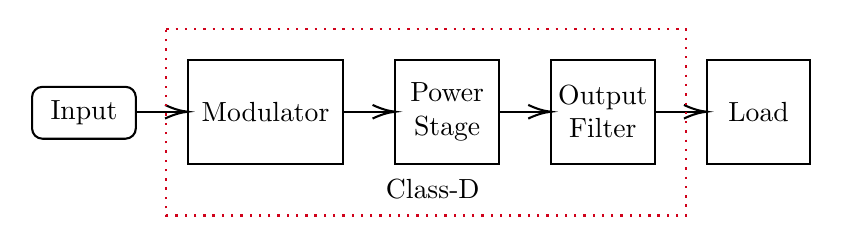
\begin{tikzpicture}[x=0.75pt,y=0.75pt,yscale=-1,xscale=1]
%uncomment if require: \path (0,117); %set diagram left start at 0, and has height of 117

%Rounded Rect [id:dp8561064043090778] 
\draw   (25,43) .. controls (25,40.24) and (27.24,38) .. (30,38) -- (70,38) .. controls (72.76,38) and (75,40.24) .. (75,43) -- (75,58) .. controls (75,60.76) and (72.76,63) .. (70,63) -- (30,63) .. controls (27.24,63) and (25,60.76) .. (25,58) -- cycle ;

%Shape: Rectangle [id:dp3490479820342707] 
\draw   (100,25) -- (175,25) -- (175,75) -- (100,75) -- cycle ;

%Shape: Rectangle [id:dp37255646201919634] 
\draw   (200,25) -- (250,25) -- (250,75) -- (200,75) -- cycle ;

%Shape: Rectangle [id:dp7847032693215759] 
\draw   (275,25) -- (325,25) -- (325,75) -- (275,75) -- cycle ;

%Shape: Rectangle [id:dp31546701870918703] 
\draw   (350,25) -- (400,25) -- (400,75) -- (350,75) -- cycle ;

%Straight Lines [id:da6350274327867016] 
\draw    (75,50) -- (98,50) ;
\draw [shift={(100,50)}, rotate = 180] [color={rgb, 255:red, 0; green, 0; blue, 0 }  ][line width=0.75]    (10.93,-3.29) .. controls (6.95,-1.4) and (3.31,-0.3) .. (0,0) .. controls (3.31,0.3) and (6.95,1.4) .. (10.93,3.29)   ;
%Straight Lines [id:da8446351183431686] 
\draw    (175,50) -- (198,50) ;
\draw [shift={(200,50)}, rotate = 180] [color={rgb, 255:red, 0; green, 0; blue, 0 }  ][line width=0.75]    (10.93,-3.29) .. controls (6.95,-1.4) and (3.31,-0.3) .. (0,0) .. controls (3.31,0.3) and (6.95,1.4) .. (10.93,3.29)   ;
%Straight Lines [id:da6769720987576957] 
\draw    (250,50) -- (273,50) ;
\draw [shift={(275,50)}, rotate = 180] [color={rgb, 255:red, 0; green, 0; blue, 0 }  ][line width=0.75]    (10.93,-3.29) .. controls (6.95,-1.4) and (3.31,-0.3) .. (0,0) .. controls (3.31,0.3) and (6.95,1.4) .. (10.93,3.29)   ;
%Straight Lines [id:da640763154281043] 
\draw    (325,50) -- (348,50) ;
\draw [shift={(350,50)}, rotate = 180] [color={rgb, 255:red, 0; green, 0; blue, 0 }  ][line width=0.75]    (10.93,-3.29) .. controls (6.95,-1.4) and (3.31,-0.3) .. (0,0) .. controls (3.31,0.3) and (6.95,1.4) .. (10.93,3.29)   ;
%Shape: Rectangle [id:dp19014479748101398] 
\draw  [color={rgb, 255:red, 208; green, 2; blue, 27 }  ,draw opacity=1 ][dash pattern={on 0.84pt off 2.51pt}] (89.69,10) -- (340,10) -- (340,100) -- (89.69,100) -- cycle ;

% Text Node
\draw (137.5,50) node   [align=left] {\begin{minipage}[lt]{51.00000000000001pt}\setlength\topsep{0pt}
\begin{center}
Modulator
\end{center}

\end{minipage}};
% Text Node
\draw (225,50) node   [align=left] {\begin{minipage}[lt]{34pt}\setlength\topsep{0pt}
\begin{center}
Power\\Stage
\end{center}

\end{minipage}};
% Text Node
\draw (300,50) node   [align=left] {\begin{minipage}[lt]{34pt}\setlength\topsep{0pt}
\begin{center}
Output\\Filter
\end{center}

\end{minipage}};
% Text Node
\draw (375,50) node   [align=left] {\begin{minipage}[lt]{34pt}\setlength\topsep{0pt}
\begin{center}
Load
\end{center}

\end{minipage}};
% Text Node
\draw (50,50.5) node   [align=left] {\begin{minipage}[lt]{34pt}\setlength\topsep{0pt}
\begin{center}
Input
\end{center}

\end{minipage}};
% Text Node
\draw (194,81) node [anchor=north west][inner sep=0.75pt]   [align=left] {Class-D};


\end{tikzpicture}

	\caption{Most basic block diagram of a class-D system}
	\label{fig:02_class_basic_blockdiagram}
\end{figure}

The most basic block diagram of a class-D system can be seen in \autoref{fig:02_class_basic_blockdiagram}. This is not in practical use, as the system lacks a feedback loop. The power stage is directly proportional to the supply level to feed a low impedance directly to the load. Therefore, any disturbances in the supply will directly degrade the output. This is why a control loop is typically connected from the output of the amplifier going to the input of the amplifier \cite{self_osc_pwm_modulators_topo_comp}. \\

In this project, a system will be implemented corresponding to the block diagram below.
\begin{figure}[htbp]
	\centering
	\tikzset{every picture/.style={line width=0.75pt}} %set default line width to 0.75pt        

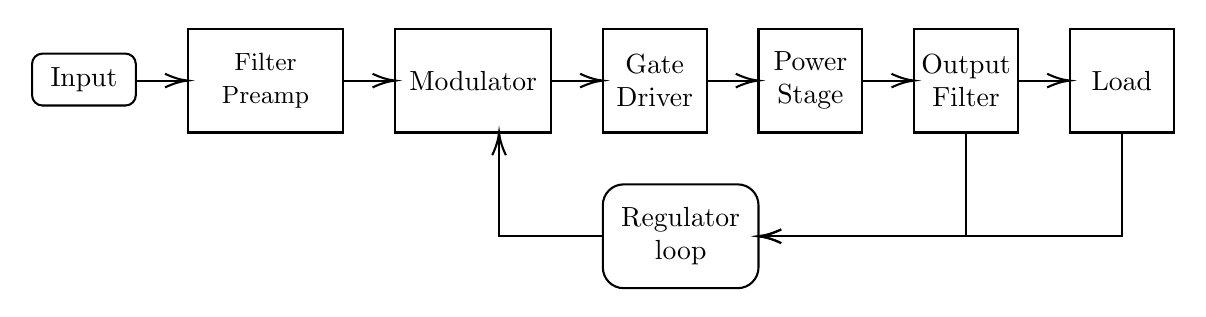
\begin{tikzpicture}[x=0.75pt,y=0.75pt,yscale=-1,xscale=1]
	%uncomment if require: \path (0,173); %set diagram left start at 0, and has height of 173
	
	%Rounded Rect [id:dp1384107767481697] 
	\draw   (25,42) .. controls (25,39.24) and (27.24,37) .. (30,37) -- (70,37) .. controls (72.76,37) and (75,39.24) .. (75,42) -- (75,57) .. controls (75,59.76) and (72.76,62) .. (70,62) -- (30,62) .. controls (27.24,62) and (25,59.76) .. (25,57) -- cycle ;
	
	%Shape: Rectangle [id:dp21588825794167765] 
	\draw   (100,25) -- (175,25) -- (175,75) -- (100,75) -- cycle ;
	
	%Shape: Rectangle [id:dp3490479820342707] 
	\draw   (200,25) -- (275,25) -- (275,75) -- (200,75) -- cycle ;
	
	%Shape: Rectangle [id:dp33842426481401633] 
	\draw   (300,25) -- (350,25) -- (350,75) -- (300,75) -- cycle ;
	
	%Shape: Rectangle [id:dp37255646201919634] 
	\draw   (375,25) -- (425,25) -- (425,75) -- (375,75) -- cycle ;
	
	%Shape: Rectangle [id:dp7847032693215759] 
	\draw   (450,25) -- (500,25) -- (500,75) -- (450,75) -- cycle ;
	
	%Shape: Rectangle [id:dp31546701870918703] 
	\draw   (525,25) -- (575,25) -- (575,75) -- (525,75) -- cycle ;
	
	%Rounded Rect [id:dp04914119895791669] 
	\draw   (300,110) .. controls (300,104.48) and (304.48,100) .. (310,100) -- (365,100) .. controls (370.52,100) and (375,104.48) .. (375,110) -- (375,140) .. controls (375,145.52) and (370.52,150) .. (365,150) -- (310,150) .. controls (304.48,150) and (300,145.52) .. (300,140) -- cycle ;
	
	%Straight Lines [id:da6350274327867016] 
	\draw    (75,50) -- (98,50) ;
	\draw [shift={(100,50)}, rotate = 180] [color={rgb, 255:red, 0; green, 0; blue, 0 }  ][line width=0.75]    (10.93,-3.29) .. controls (6.95,-1.4) and (3.31,-0.3) .. (0,0) .. controls (3.31,0.3) and (6.95,1.4) .. (10.93,3.29)   ;
	%Straight Lines [id:da5761730573744579] 
	\draw    (175,50) -- (198,50) ;
	\draw [shift={(200,50)}, rotate = 180] [color={rgb, 255:red, 0; green, 0; blue, 0 }  ][line width=0.75]    (10.93,-3.29) .. controls (6.95,-1.4) and (3.31,-0.3) .. (0,0) .. controls (3.31,0.3) and (6.95,1.4) .. (10.93,3.29)   ;
	%Straight Lines [id:da8446351183431686] 
	\draw    (275,50) -- (298,50) ;
	\draw [shift={(300,50)}, rotate = 180] [color={rgb, 255:red, 0; green, 0; blue, 0 }  ][line width=0.75]    (10.93,-3.29) .. controls (6.95,-1.4) and (3.31,-0.3) .. (0,0) .. controls (3.31,0.3) and (6.95,1.4) .. (10.93,3.29)   ;
	%Straight Lines [id:da8956311563709014] 
	\draw    (350,50) -- (373,50) ;
	\draw [shift={(375,50)}, rotate = 180] [color={rgb, 255:red, 0; green, 0; blue, 0 }  ][line width=0.75]    (10.93,-3.29) .. controls (6.95,-1.4) and (3.31,-0.3) .. (0,0) .. controls (3.31,0.3) and (6.95,1.4) .. (10.93,3.29)   ;
	%Straight Lines [id:da6769720987576957] 
	\draw    (425,50) -- (448,50) ;
	\draw [shift={(450,50)}, rotate = 180] [color={rgb, 255:red, 0; green, 0; blue, 0 }  ][line width=0.75]    (10.93,-3.29) .. controls (6.95,-1.4) and (3.31,-0.3) .. (0,0) .. controls (3.31,0.3) and (6.95,1.4) .. (10.93,3.29)   ;
	%Straight Lines [id:da640763154281043] 
	\draw    (500,50) -- (523,50) ;
	\draw [shift={(525,50)}, rotate = 180] [color={rgb, 255:red, 0; green, 0; blue, 0 }  ][line width=0.75]    (10.93,-3.29) .. controls (6.95,-1.4) and (3.31,-0.3) .. (0,0) .. controls (3.31,0.3) and (6.95,1.4) .. (10.93,3.29)   ;
	%Straight Lines [id:da8759504451760138] 
	\draw    (475,75) -- (475,125) -- (377,125) ;
	\draw [shift={(375,125)}, rotate = 360] [color={rgb, 255:red, 0; green, 0; blue, 0 }  ][line width=0.75]    (10.93,-3.29) .. controls (6.95,-1.4) and (3.31,-0.3) .. (0,0) .. controls (3.31,0.3) and (6.95,1.4) .. (10.93,3.29)   ;
	%Straight Lines [id:da9426589856839147] 
	\draw    (550,75) -- (550,125) -- (377,125) ;
	\draw [shift={(375,125)}, rotate = 360] [color={rgb, 255:red, 0; green, 0; blue, 0 }  ][line width=0.75]    (10.93,-3.29) .. controls (6.95,-1.4) and (3.31,-0.3) .. (0,0) .. controls (3.31,0.3) and (6.95,1.4) .. (10.93,3.29)   ;
	%Straight Lines [id:da6532117977416998] 
	\draw    (300,125) -- (250,125) -- (250,77) ;
	\draw [shift={(250,75)}, rotate = 450] [color={rgb, 255:red, 0; green, 0; blue, 0 }  ][line width=0.75]    (10.93,-3.29) .. controls (6.95,-1.4) and (3.31,-0.3) .. (0,0) .. controls (3.31,0.3) and (6.95,1.4) .. (10.93,3.29)   ;
	
	
	% Text Node
	\draw (50,49.5) node   [align=left] {\begin{minipage}[lt]{34pt}\setlength\topsep{0pt}
			\begin{center}
				Input
			\end{center}
			
	\end{minipage}};
	% Text Node
	\draw (137.5,50) node   [align=left] {\begin{minipage}[lt]{51.00000000000001pt}\setlength\topsep{0pt}
			\begin{center}
				{\small Filter}\\{\small Preamp}
			\end{center}
			
	\end{minipage}};
	% Text Node
	\draw (237.5,50) node   [align=left] {\begin{minipage}[lt]{51.00000000000001pt}\setlength\topsep{0pt}
			\begin{center}
				Modulator
			\end{center}
			
	\end{minipage}};
	% Text Node
	\draw (325,50) node   [align=left] {\begin{minipage}[lt]{34pt}\setlength\topsep{0pt}
			\begin{center}
				Gate Driver
			\end{center}
			
	\end{minipage}};
	% Text Node
	\draw (400,50) node   [align=left] {\begin{minipage}[lt]{34pt}\setlength\topsep{0pt}
			\begin{center}
				Power\\Stage
			\end{center}
			
	\end{minipage}};
	% Text Node
	\draw (475,50) node   [align=left] {\begin{minipage}[lt]{34pt}\setlength\topsep{0pt}
			\begin{center}
				Output\\Filter
			\end{center}
			
	\end{minipage}};
	% Text Node
	\draw (550,50) node   [align=left] {\begin{minipage}[lt]{34pt}\setlength\topsep{0pt}
			\begin{center}
				Load
			\end{center}
			
	\end{minipage}};
	% Text Node
	\draw (337.5,125) node   [align=left] {\begin{minipage}[lt]{51.00000000000001pt}\setlength\topsep{0pt}
			\begin{center}
				Regulator\\loop
			\end{center}
			
	\end{minipage}};
	
	
\end{tikzpicture}
	\caption{Overview block diagram of class-D circuit}
	\label{fig:02_circuit_block_diagram}
\end{figure}
As seen in \autoref{fig:02_circuit_block_diagram} the input signal will go directly into an input filter and preamp. This block consists of a subcircuit with a filter combined with a pre-amp and level-shifting circuit combined in one. This block takes an unbalanced line-level signal from an audio source and filters undesirable frequencies out of the input signal and level-level shifts it to a desired operating point in the centre of the supply voltage DR. \\
In the second stage, the filtered and shifted signal enters the modulator, where it will be converted to a logic-level pulse-train modulated in a PWM scheme (a binary representation of the audio). This logic-level signal is sent to the gate driver circuit that controls the power stage. At the power stage, the logic-level signal is amplified to a high-amplitude signal through the switching operation.\\
After the power stage, the high-amplitude binary signal is sent through the output filter, which converts the modulated pulse-train back to its original form. In practice, this is done by a low-pass filter which removes the high-frequency components of the PWM signal and leaves an amplified version of the original input signal to pass to the load (in this application, a speaker). \\
In this design, a control loop (or regulator loop) is connected from the output stage and load and back to the modulator stage to control the amplification of the system using feedback.

\section{Preamplifier and Input Filter} \label{sec:theory_filter_preamp}

\begin{figure}[htbp]
	\centering
	\begin{circuitikz}
		%\begin{tikzpicture}
	%\draw (0,0) 	node[op amp, noinv input up](opamp){};
	% C_1 and R_1
	%\draw (opamp.+) to[R,l=$R_1$,*-o] ++(0,2.5) node[above]{$V_{ref}$};
	%\draw (opamp.+) to[C,l_=$C_1$,-o] ++(-2.5,0) node[left](V_in){$V_{in}$};
	% R_2, R_3, and C_2
	%\draw (opamp.-) to[short,-*] ++(0,-1) node(node_m){};
	%\draw (node_m) to[R,l_=$R_3$,*-o] ++(-2.5,0) node[left]{$V_{ref}$};
	
	%\draw (node_m) to[R,l=$R_2$,-*] ++(2.5,0) -| (opamp.out);
	%\draw (node_-) to[short] ++(0,-1.25) to[C,l=$C_2$] ++(2.5,0) -| (opamp.out);
	
	% V_out
	%\draw (opamp.out) to[short,*-o] ++(1,0) node[right]{$V_{out}$};
	%\draw (opamp.out) -| (node_out);
%\end{tikzpicture}

\node   (comp)  [op amp, noinv input up, right, anchor=-] {};
	% C_1 and R_1
\draw (comp.+) to[R,l=$R_1$,*-o] ++(0,2.5) node[above]{$V_{\mathrm{ref}}$};
\draw (comp.+) to[C,l_=$C_3$,-o] ++(-2.5,0) node[left](V_in){$V_{in}$};
	% R_2, R_3, and C_2
\draw (comp.-) to[short,-] ++(0,-1) node(node_m){};
\draw (node_m) to[R,l_=$R_3$,*-o] ++(-2.38,0) node[left]{$V_{\mathrm{ref}}$};

\draw (node_m) to[R,l=$R_2$,-*] ++(2.38,0) -| (comp.out);
\draw (node_m) to[short] ++(0,-1.25) to[C,l=$C_2$] ++(2.38,0) -| (comp.out);

	% V_out
\draw (comp.out) to[short,*-o] ++(1,0) node[right]{$V_{\mathrm{out}}$};
	\end{circuitikz}
	\caption{Part-schematic of Filter and input preamp}
	\label{fig:02_part_filter_preamp}
\end{figure}

The part-schematic for the input filter can be seen in \autoref{fig:02_part_filter_preamp} and is used to attenuate undesired frequencies outside the audio frequency range. Fundamentally, it is a non-inverting amplifier coupling with some added filters. There is also a DC bias point $V_{ref}$ which will operate the audio output of the preamplifier to a bias point of $V_{ref}$. The input capacitor $C_{1}$ is intentionally used for blocking any DC component on the input prior to the level-shift. In a practical sense, this sub-circuit works as a band-pass filter with a high-pass filter ($C_{1}$, $R_{1}$) on the positive input and a low-pass filter ($C_{2}$, $R_{2}$) on the negative input of the operational amplifier. The fundamental equations for each cut-off in the part-filter can be seen in \autoref{eq:preamp_cut-off-filters}.

\begin{subequations} \label{eq:preamp_cut-off-filters}
	\begin{equation} \label{eq:preamp_cut-off-filtersa}
		f_{\mathrm{hp}} = \frac{1}{2 \pi \cdot R_{1}C_{1}}
	\end{equation}
	\begin{equation} \label{eq:preamp_cut-off-filtersb}
		f_{\mathrm{lp}} = \frac{1}{2 \pi \cdot R_{2}C_{2}}
	\end{equation}
\end{subequations}

With the amplification factor given by the voltage divider in the feedback network as \autoref{eq:preamp_gain}.

\begin{equation} \label{eq:preamp_gain}
	A_{v} = 1 + \frac{R_{2}}{R_{3}}
\end{equation}

\section{Modulator}
The modulator in a class-D amplifier is the module that converts the continuous audio signal to a rail level discrete pulse coded signal. Generally, using pulse coded signals a PWM method is utilised. The audio input is coded into a PWM signal by comparison of a triangle-shaped carrier waveform. A comparator will set the output to HIGH when the audio signal has a higher potential than the carrier waveform and a LOW will be set on the output when the audio signal is lower than the carrier waveform. The portion of time where the modulator has a high output to a single period is called the DUTY cycle.
\begin{figure}[htbp]
	\centering
	\begin{circuitikz}
			\draw (0,0) 	node[op amp, noinv input up](opamp){}
	(opamp.+) to [sV, l_=$V_{\mathrm{in}}$, -] ++(-3,0) node[ground](GND){}
	(opamp.-) to [tV, l=$V_{\mathrm{carrier}}$, -] ++(-2,0) node[ground](GND){}

	%(opamp.out) to[short] ++(0.2, 0)
	(opamp.out) to[right,-o] ++(0.2,0) node[right](V_pwm){$V_{\mathrm{pwm}}$};

	\end{circuitikz}
	\caption{Simple comparator modulator}
	\label{fig:02_comparator_modulator}
\end{figure}
Referring to \autoref{fig:02_comparator_modulator}, the modulator comparator is connected to its input signal sinusoidal signal on its positive terminal and the carrier signal on the negative terminal, providing a PWM signal on the output with a fixed PWM frequency. This standard configuration entails an open-loop system and no error-correction. Furthermore, the fixed frequency can increase EMI in the circuit \cite{sw_freq_variations_and_EMI_prop_in_selfosc_classD_amps}. \\

\begin{figure}[htbp]
	\centering
	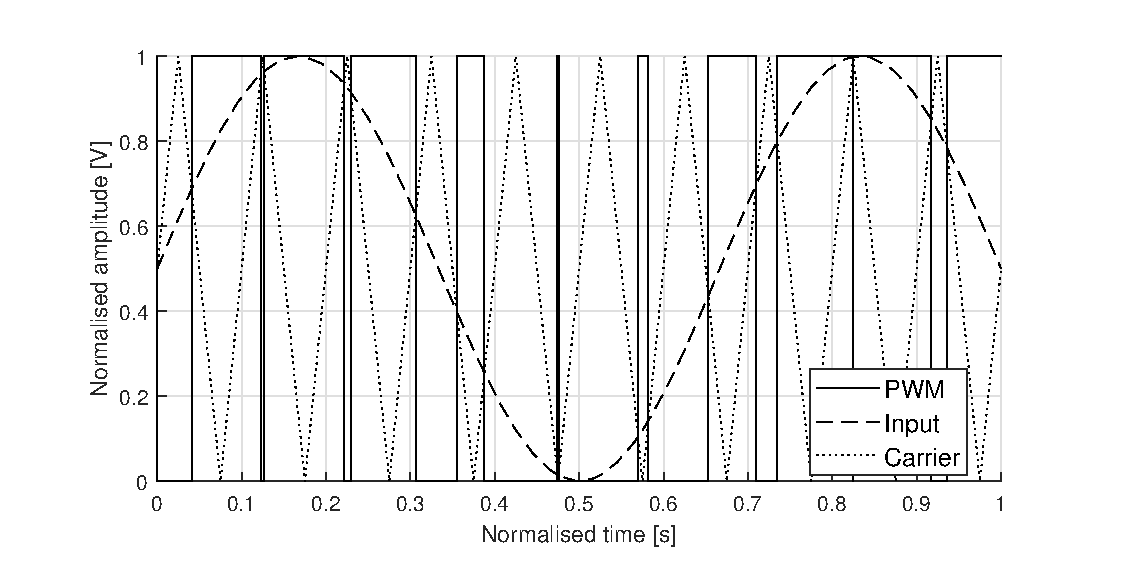
\includegraphics[width=0.9\textwidth]{Theory/modulator_pwm_example_black.eps}
	\caption{Typical PWM modulation scheme example}
	\label{fig:pwm_example}
\end{figure}
Seen in \autoref{fig:pwm_example} is a typical PWM operation. The input and carrier waveform is compared to give a PWM output as described in \autoref{fig:02_comparator_modulator} according to \Cref{lst:simple_modulator.m,fig:pwm_modulator_sim}.

It is chosen to utilise a self-oscillating modulation scheme for this project. This modulation scheme is different as it does not require an externally clocked carrier waveform to modulate the digital pulses on the comparator sub-circuit. Instead, the reference signal is added together with the feedback signal and fed into a hysteretic comparator. \\
For this system, the AIM design is based on the article \cite{Comp_Simp_selfosc_PWM_mod}. 

\subsection{Astable Integrating Modulator}

\begin{figure}[htbp]
	\centering
	\begin{circuitikz}
		
	% Drawn op-amp
	\draw (0,0) 	node[op amp, noinv input up](opamp){}
	(opamp.+) node[left] {$V_{\mathrm{hw}}$}
	(opamp.-) node[left] {$V_{c}$};
	% V_pwm putput
	\draw (opamp.out)	to[short,*-o] ++(.5,0) node[right](V_pwm){$V_{\mathrm{pwm}}$};
	% R_1 & R_2
	\draw (opamp.+) to[short,-*] ++(0,1) node(R1R2){};
	\draw (R1R2) ++(-2.25,0) node[left](V_ref){$V_{\mathrm{ref}}$} to[R,l=$R_{1}$,o-] (R1R2);
	\draw (R1R2) 	to[R,l=$R_{2}$] ++(2.25,0) -| (opamp.out);
	% R_in & R_fb
	\draw (opamp.-) to[short,-*] ++(0,-1) node(RinRfb){};
	\draw (RinRfb) ++(-2.25,0) node[left](V_in){$V_{\mathrm{in}}$} to[R,l=$R_{\mathrm{in}}$,o-] (RinRfb);
	\draw (RinRfb) 	to[R,l=$R_{\mathrm{fb}}$] ++(2.25,0) -| (opamp.out);
	% Capacitor C
	\draw (RinRfb) to[C,l=$C_{1}$] ++(0,-1.5) node[tlground](GND){};
	\end{circuitikz}
	\caption{Part-schematic of modulator}
	\label{fig:02_modulator_circuit}
\end{figure}

The part-schematic for the AIM sub-circuit can be seen in \autoref{fig:02_modulator_circuit}. Other than the OP-AMP, the sub-circuit consists of a voltage divider ($R_{1}$ and $R_{2}$) and a charging circuit with $R_{\mathrm{in}}$, $R_{\mathrm{fb}}$ and $C_{1}$. $V_{\mathrm{in}}$ represents the continuous audio signal from the pre-amplifier and filter. $V_{\mathrm{ref}}$ is a reference voltage. $V_{\mathrm{pwm}}$ represents the modulated output signal. This system fundamentally works by employing a filter on the output to generate the carrier waveform in a feedback configuration \cite{Comp_Simp_selfosc_PWM_mod}. The system is operated in a perpetual self-oscillating state by intentionally introducing a hysteresis window or a \SI{180}{\degree} phase shift in the feedback network \cites{simp_PWM_mod_topo_with_excellent_dynamic_behavior,putzey_simple_self_osc_amp_filter_control}. Since the feedback network results in a variable switching frequency, which infers a reduction in EMI \cite{sw_freq_variations_and_EMI_prop_in_selfosc_classD_amps}.
In this project derived equations from \cites{Comp_Simp_selfosc_PWM_mod,multivar_ctrl_loops_for_SM_audio_systems,soren_simonsen} will be used. \\
The PWM signal $V_{\mathrm{pwm}}$ has the two states HIGH ($V_{H}$) and LOW ($V_{L}$), both of which are defined in the expressions below.
\begin{subequations} \label{eq:pwm_states}
	\begin{equation} \label{eq:pwm_states_a}
		V_{H} = V_{\mathrm{ref}} + \frac{V_{\mathrm{out}}}{2}
	\end{equation}
	\begin{equation} \label{eq:pwm_states_b}
		V_{L} = V_{\mathrm{ref}} - \frac{V_{\mathrm{out}}}{2}
	\end{equation}
\end{subequations}
Where $V_{\mathrm{ref}}$ is the reference voltage and $V_{\mathrm{out}} = \left( V_{H} - V_{L} \right)$ is the output voltage span of $V_{\mathrm{pwm}}$. \\
Additionally, the hysteresis window has threshold voltages $V_{\mathrm{th}_{H}}$ (upper) and $V_{\mathrm{th}_{L}}$ (lower) described as:
\begin{subequations} \label{eq:hysteresis_window}
	\begin{equation} \label{eq:hysteresis_window_a}
		V_{\mathrm{th}_{H}} = V_{\mathrm{hw}} \cdot \frac{V_{H} - V_{\mathrm{ref}}}{V_{H} - V_{L}} + V_{\mathrm{ref}}
	\end{equation}
	\begin{equation} \label{eq:hysteresis_window_b}
		V_{\mathrm{th}_{L}} = V_{\mathrm{hw}} \cdot \frac{V_{L} - V_{\mathrm{ref}}}{V_{H} - V_{L}} + V_{\mathrm{ref}}
	\end{equation}
\end{subequations}
Where $V_{\mathrm{hw}}$ is the hysteresis window width.

The switching frequency $f_{\mathrm{sw}}$ of output signal $V_{\mathrm{pwm}}$ is expressed by:
\begin{equation}
	f_{\mathrm{sw}} = \frac{1}{t_{\mathrm{high}} + t_{\mathrm{low}}} = \frac{1}{-C \cdot R_{t} \cdot \ln \left( \frac{(V_{\mathrm{hw}} - 2V_{th_{H}}) (2V_{th_{L}} + V_{\mathrm{hw}})}{ (V_{\mathrm{hw}} - 2V_{th_{L}}) (2V_{th_{H}}+ V_{\mathrm{hw}}) } \right) }
\end{equation}
And DUTY cycle given by:
\begin{equation}
	D = \frac{t_{\mathrm{high}}}{t_{\mathrm{high}} + t_{\mathrm{low}}} = \frac{\ln \left( \frac{2V_{th_{H}} - V_{\mathrm{hw}}}{2V_{th_{H}} - V_{\mathrm{hw}}} \right) }{\ln \left( \frac{(V_{\mathrm{hw}} - 2V_{th_{H}}) (2V_{th_{L}} + V_{\mathrm{hw}})}{ (V_{\mathrm{hw}} - 2V_{th_{L}}) (2V_{th_{H}}+ V_{\mathrm{hw}}) } \right)}
\end{equation}
The timing variables $t_{\mathrm{high}}$ and $t_{\mathrm{low}}$ are expressed by the following:
\begin{subequations} \label{eq:aim_timing}
	\begin{equation} \label{eq:aim_timing_a}
		t_{\mathrm{high}} = \tau \cdot \ln \left( \frac{V_{c_{H}} - V_{\mathrm{th}_{L}}}{V_{c_{H}} - V_{\mathrm{th}_{H}}} \right) 
	\end{equation}
	\begin{equation} \label{eq:aim_timing_b}
		t_{\mathrm{low}} = -\tau \cdot \ln \left( \frac{V_{c_{L}} - V_{\mathrm{th}_{L}}}{V_{c_{L}} - V_{\mathrm{th}_{H}}} \right)
	\end{equation}
\end{subequations}
Where carrier waveform limits $V_{c_{H}}$ and $V_{c_{L}}$ are given by:
\begin{subequations} \label{eq:carrier_waveform}
	\begin{equation} \label{eq:carrier_waveform_a}
		V_{c_{H}} = V_{\mathrm{in}} + \frac{V_{\mathrm{span}} \cdot \left( V_{H} - V_{\mathrm{in}} \right) + V_{\mathrm{hw}} \cdot \left( V_{H} - V_{\mathrm{in}} \right)  }{V_{H} - V_{L} + V_{\mathrm{span}}}
	\end{equation}
	\begin{equation} \label{eq:carrier_waveform_b}
		V_{c_{L}} = V_{\mathrm{in}} + \frac{V_{\mathrm{span}} \cdot \left( V_{L} - V_{\mathrm{in}} \right) + V_{\mathrm{hw}} \cdot \left( V_{L} - V_{\mathrm{in}} \right)  }{V_{H} - V_{L} + V_{\mathrm{span}}}
	\end{equation}
\end{subequations}
Where $V_{\mathrm{span}}$ is the input voltage range of $V_{\mathrm{in}}$

The time constant $\tau$ is defined by the feedback network containing $R_{\mathrm{in}}$, $R_{\mathrm{fb}}$ and $C_{1}$ and is given by:
\begin{equation} \label{eq:aim_time_constant}
	\tau = R_{t} \cdot C_{1}
\end{equation}
Where $R_{t}$ is the Thevenin resistance of the feedback network.

%\comment{
To determine the Thevenin resistance the circuit is evaluated with no input, at $V_{\mathrm{in}} = V_{\mathrm{ref}}$. That means the self-oscillating switching frequency becomes the idle frequency $f_{\mathrm{idle}}$. 
Then the expression for the Thevenin resistance becomes:
\begin{equation} \label{eq:modulator_thevenin_resistance}
	R_t = \frac{1}{f_{\mathrm{idle}} C_{1} \ln{ \left( \frac{(V_{c_{H}} - V_{\mathrm{th}_{L}})(V_{c_{L}} - V_{\mathrm{th}_{H}})}{(V_{c_{H}} - V_{\mathrm{th}_{H}})(V_{c_{L}} - V_{\mathrm{th}_{L}})} \right) }}
\end{equation}

Where $V_{c_{H}}$ and $V_{c_{L}}$ are carrier waveform limits found in \autoref{eq:carrier_waveform}. The expressions for $R_{\mathrm{in}}$ and $R_{\mathrm{fb}}$ are desired.
%}
The Thevenin resistance is expressed by a parallel connection of the following:
\begin{equation}
	R_{t} = R_{\mathrm{in}} \parallel R_{\mathrm{fb}} = \frac{R_{\mathrm{in}} \cdot R_{\mathrm{fb}}}{R_{\mathrm{in}} + R_{\mathrm{fb}}}
\end{equation}

The $k_{2}$ of $R_{\mathrm{in}}$ and $R_{\mathrm{fb}}$ voltage divider can be described as:
\begin{equation} \label{eq:k2_voltage_divider}
	k_{2} = \frac{V_{c_{H}} - V_{c_{L}}}{V_{H} - V_{L}} = \frac{V_{c_{H}} - V_{c_{L}}}{V_{\mathrm{out}}}
\end{equation}
By inserting from \autoref{eq:carrier_waveform} into \autoref{eq:k2_voltage_divider} and simplifying the expression becomes \autoref{eq:modulator_k2_voltage_divider}, the derived expression becomes \Cref{eq:modulator_rfb_rin_a,eq:modulator_rfb_rin_b}.
\begin{equation} \label{eq:modulator_k2_voltage_divider}
	k_{2} = \frac{V_{\mathrm{span}} + V_{\mathrm{hw}}}{V_{\mathrm{span}} + V_{\mathrm{out}}} = \frac{R_{\mathrm{in}}}{R_{\mathrm{in}} + R_{\mathrm{fb}}} \Longrightarrow 
\end{equation}
\begin{subequations} \label{eq:modulator_rfb_rin}
	\begin{equation} \label{eq:modulator_rfb_rin_a}
		R_{\mathrm{fb}} = R_{t} \cdot \frac{V_{\mathrm{span}} + V_{\mathrm{out}}}{V_{\mathrm{span}} + V_{\mathrm{hw}}}
	\end{equation}
	\begin{equation} \label{eq:modulator_rfb_rin_b}
		R_{\mathrm{in}} = \frac{R_{\mathrm{fb}} \cdot R_{t}}{R_{\mathrm{fb}} - R_{t}}
	\end{equation}
\end{subequations}
Where the hysteresis $V_{\mathrm{hw}}$ is expressed by the voltage divider in $R_{1}$ and $R_{2}$:
\begin{equation}
	V_{\mathrm{hw}} = \frac{R_{1}}{R_{1} + R_{2}} \cdot V_{\mathrm{out}}
\end{equation}

Finally, the two expression to determine the the two resistor values $R_{1}$ and $R_{2}$ are obtained:
\begin{subequations} \label{eq:aim_resistor_expression2}
	\begin{equation} \label{eq:aim_resistor_expression2_a}
		R_{1} = \frac{V_{\mathrm{hw}}}{V_{\mathrm{out}} - V_{\mathrm{hw}}} \cdot R_{2}
	\end{equation}
	\begin{equation} \label{eq:aim_resistor_expression2_b}
		R_{2} = \left( \frac{V_{\mathrm{out}}}{V_{\mathrm{hw}}} -1 \right) \cdot R_{1}
	\end{equation}
\end{subequations}
It is noted that in \autoref{eq:aim_resistor_expression2} that if a resistor value is chosen, the other can be calculated.

\section{Gate Driver}
\begin{figure}[H]
	\centering
	\begin{circuitikz}
			\draw (0,0) to[sqV,l=$V_{\mathrm{pwm}}$] ++(0,-2) node[tlground]{};
	\draw (0,0) to[short,.-*] ++(1.5,0) node(PWM){};
	\draw (PWM) to[short] ++(0,.75) ++(2.5,0) to[sDo,l_=$D$] ++(-2.5,0) ++(2.5,0) to[short,-*] ++(0,-.75) node(node_DR){};
	\draw (PWM) to[short] ++(0,-.75) to[vR,l=$R_{\mathrm{dt}}$] ++(2.5,0) to[short] (node_DR);
	\draw (node_DR){} to[short,-*] ++(1,0) node(C_N){} to[short,-] ++(1,0) node[right](out){};
	\draw (C_N) to[C,l=$C_{\mathrm{dt}}$] ++(0,-2) node[tlground]{};
	
	\draw [thick] (6,-0.5) coordinate (u1) rectangle ++(2.2,1); % shape
	\draw [pin] (u1) ++ (0,0.5) coordinate (u1 in) node[right]{Gate Driver};
	%node[above left]{5}; % CON
	%\draw [pin] (u1) ++ (0,1) coordinate (u1 tri)
	%node[right]{TRI}
	%node[above left]{2}; % TRI
	%\draw [pin] (u1) ++ (0,1.5) coordinate (u1 thr)
	%node[right]{THR}
	%node[above left]{6}; % THR
	%\draw [pin] (u1) ++ (0,2) coordinate (u1 dis)
	%node[right]{DIS}
	%node[above left]{7}; % DIS
	%\draw [pin] (u1) ++ (0,2.5) coordinate (u1 rst) 
	%node[right]{RST}
	%node[above left]{4}; % RST
	%\draw [pin] (u1) ++ (1,3) coordinate (u1 vcc)
	%node[below]{VCC}
	%node[above left]{8}; % VCC
	%\draw [pin] (u1) ++ (1,0) coordinate (u1 gnd)
	%node[above]{GND}
	%node[below left]{1}; % GND
	%\draw [pin] (u1) ++ (2,2.5) coordinate (u1 out)
	%node[left]{OUT};
	%node[above right]{3}; % OUT
	%\draw (u1) ++ (2,0);
	%node[right]{\ctikzlabel{$U_1$}{NE555}}; % NE555P
	
	\draw (8.2,0) to[short,-o] ++(1,0) node[right]{$V_{\mathrm{G}}$};
	\end{circuitikz}
	\caption{Part-schematic of the dead-time and gate driver}
	\label{fig:deadtime_gate}
\end{figure}

The gate driver subcircuit is based on a design from \cite{nagy_special_course}. It is comprised of an integrated circuit from Texas Instruments, LM5113 \cite{lm5113} and a dead-time circuit.
This subcircuit is responsible for the timing of the gate drive and ripple present in the drive signal before it reaches the power stage. The LM5113 IC has built-in bootstrap port to drive the MOSFETs HIGH \cite{onsemi_boostrap} and two output ports, one for each gate on the half-bridge. The IC does not include a built-in dead-time circuit, which is why an external one is present. Using a variable resistor, the timing of the PWM signal can be adjusted and tuned to the desired dead-time in the HIGH and LOW side on the power stage. It consists of a simple RC-network and a Schottky diode. \\
The external dead-time circuit seen in \autoref{fig:deadtime_gate} on the left side leading into the gate driver. The output of the gate driver $V_{G}$ is connected to the gate of the power stage switch. The voltage across the capacitor $C_{\mathrm{dt}}$ is equal to the input voltage of the gate drive IC and is described by:

\begin{equation} \label{eq:deadtime_voltage}
	V_{C} = V_{\mathrm{pwm}} \cdot e^{-\frac{t}{R_{\mathrm{dt}} C_{\mathrm{dt}}}}
\end{equation}

When $V_{C}$ in \autoref{eq:deadtime_voltage} reaches the threshold voltage of the gate driver input, the output $V_{G}$ will switch to a HIGH state. Effectively, controlling the charge time of the capacitor means adjusting the time it takes for the gate driver to flip state. 

\section{Power Stage} \label{sec:power_stage}
\begin{figure}[htbp]
	\centering
	\begin{subfigure}[b]{0.5\textwidth}
		\centering
		\begin{circuitikz}[>=Triangle, scale=0.8, font=\footnotesize]
			\ctikzset{bipoles/length=14mm}               % <-- smaller bipole elements
			%\begin{circuitikz} [>=Triangle]
% MIDDLE
%\begin{scope} %[blue]
%	% Resistor
%	\draw (-1,0) node[](left_R){} to[] (0.5,0) node[](right_R){};
%	% Filter cap
%	%\draw (left_R) 	node[]{}	to[short] 	++(0,-1.5) 	node(left_C){};
%	%\draw (right_R) node[]{} 	to[short]	++(0,-1.5) 	node(right_C){};
%	%\draw (left_C) to[C,l=$C_{f}$] (right_C);
%	\draw (left_R) node[circ]{} to[C,l=$C_{f}$] ++(0,-1.5) node[ground]{};
%	\draw (right_R) to[R,l=$R_{f}$] ++(0,-1.5) node[ground]{};
%	%\draw (0,-1.5) to[short,*-] ++ node[]{};
%	%\draw to[short, -] ++(0.5,-1.5) node[ground]{};
%	% Left inductor
%	\draw (left_R)
%	++(-2,0) node[](left_L){}
%	to[L,l=$L_{ind}$] (left_R);
%\end{scope}
%% LEFT SIDE
%\begin{scope} %[red]
%	% Top FET
%	\draw (left_L) 
%	to[Tnmos,n=T1] ++(0,3) node[tground](left_VD){} node[above]{$V_{DD}$};
%	\draw (T1.G) node[left]{$q$} ++(+1.2,0) node[]{$Q_1$};
%	% Bottom FET
%	\draw (left_L) ++(0,-3)
%	node[tground](left_VS){} node[below]{$V_{SS}$}
%	to[Tnmos,n=T2] ++(0,3) node[circ]{};
%	\draw (T2.G) node[left]{$\bar{q}$} ++(+1.2,0) node[]{$Q_2$};
%\end{scope}


%\draw (3.00, -5.77) node[Tnmos](nmos1){$Q_{1}$};
%\draw (3.00, -2.23) node[Tnmos](nmos2){$Q_{1}$};
%\draw (nmos1.B) to[short] (1, -5.77) ;
%\draw (nmos1.E) node[vee]{$V_{DD}$} ;
%\draw (nmos2.E) to[short] (nmos1.C) ;
%\draw (nmos2.B) to[short] (1, -2.23) ;
%\draw (nmos2.C) node[vee ,rotate=180]{$V_{SS}$} ;
%\draw (6, -6) node[ground]{} ;
%\draw (3, -4) to[L, l=$L_{\mathrm{ind}}$, *-*] ++(2, 0) coordinate(point1) to[C, l=$C_{f}$, *-] ++(0, -2) coordinate(point2) ;
%\draw (point1) to[short, *-] ++(2, 0) to[R, l=$R_{f}$] ++(0, -2) to[short] (point2) ;
\draw (3.00, -5.77) node[nmos](nmos1){$Q_{2}$};
\draw (3.00, -2.23) node[nmos](nmos2){$Q_{1}$};
\draw (nmos1.B) to[short, -o] (1.7, -5.77) node[left]{$\bar{q}$};
\draw (nmos1.E) node[vee]{} node[below, yshift=-0.35cm]{$V_{\mathrm{SS}}$} ;
\draw (nmos2.E) to[short] (nmos1.C) ;
\draw (nmos2.B) to[short, -o] (1.7, -2.23) node[left]{$q$};
\draw (nmos2.C) node[vcc]{} node[above, yshift=0.35cm]{$V_{\mathrm{DD}}$} ;
\draw (6, -6) node[ground]{} ;
\draw (3, -4) to[L, l=$L_{\mathrm{ind}}$, *-*] ++(2, 0) coordinate(point1) to[C, l=$C_f$, *-] ++(0, -2) coordinate(point2) ;
\draw (point1) to[short, *-] ++(2, 0) to[R, l=$R_f$] ++(0, -2) to[short] (point2) ;
		\end{circuitikz}
		\subcaption{Half-bridge}
		\label{fig:power_stage_halfbridge}
	\end{subfigure}%
	\begin{subfigure}[b]{0.5\textwidth}
		\centering
		\begin{circuitikz}[>=Triangle, scale=0.8, font=\footnotesize]
			\ctikzset{bipoles/length=14mm}               % <-- smaller bipole elements
			%\begin{circuitikz} [>=Triangle]
% MIDDLE
%\begin{scope} %[blue]
%	% Resistor
%	\draw (-1,0) node[](left_R){} to[R,l=$R_{BTL}$] (1,0) node[](right_R){};
%	% Filter cap
%	\draw (left_R) 	node[circ]{}	to[short] 	++(0,-1.5) 	node(left_C){};
%	\draw (right_R) node[circ]{} 	to[short]	++(0,-1.5) 	node(right_C){};
%	\draw (left_C) to[C,l=$C_{BTL}$] (right_C);
%	% Left inductor
%	\draw (left_R)
%	++(-2,0) node[](left_L){}
%	to[L,l=$L_{ind}$] (left_R);
%	% Right inductor
%	\draw (right_R)
%	to[L,l=$L_{ind}$] ++(2,0) node[](right_L){};
%\end{scope}
%% LEFT SIDE
%\begin{scope} %[red]
%	% Top FET
%	\draw (left_L) 
%	to[Tnmos,n=T1] ++(0,3) node[tground](left_VD){} node[above]{$V_{DD}$};
%	\draw (T1.G) node[left]{$q$} ++(+1.2,0) node[]{$Q_1$};
%	% Bottom FET
%	\draw (left_L) ++(0,-3)
%	node[tlground](left_VS){} %node[below]{$V_S$}
%	to[Tnmos,n=T2] ++(0,3) node[circ]{};
%	\draw (T2.G) node[left]{$\bar{q}$} ++(+1.2,0) node[]{$Q_2$};
%\end{scope}
%% RIGHT SIDE
%\begin{scope} %[green]
%	% Top FET
%	\draw (right_L) 
%	to[Tnmos,mirror,n=T3] ++(0,3) node[tground](right_VD){} node[above]{$V_{DD}$};
%	\draw (T3.G) node[right]{$\bar{q}$} ++(-1.2,0) node[]{$Q_3$};
%	% Bottom FET
%	\draw (right_L) ++(0,-3)
%	node[tlground](right_VS){} %node[below]{$V_S$}
%	to[Tnmos,mirror,n=T4] ++(0,3) node[circ]{};
%	\draw (T4.G) node[right]{$q$} ++(-1.2,0) node[]{$Q_4$};
%\end{scope}

%\draw (9.00, -5.77) node[nmos, rotate=180](nmos1){};
%\draw (9.00, -2.23) node[nmos, rotate=180](nmos2){};
%\draw (3.00, -5.77) node[nmos](nmos3){};
%\draw (3.00, -2.23) node[nmos](nmos4){};
%\draw (nmos1.E) to[short, -*] ++(0, 1) coordinate(point1) to[short, *-] (nmos2.C) ;
%\draw (nmos1.B) to[short, -o] (10.3, -5.77) node[right]{$q$};
%\draw (nmos1.C) node[ground]{} ;
%\draw (nmos2.B) to[short, -o] (10.3, -2.23) node[right]{$\bar{q}$};
%\draw (nmos2.E) node[vcc]{} node[above, yshift=0.3cm]{$V_{\mathrm{DD}}$};
%\draw (nmos3.B) to[short, -o] (1.7, -5.77) node[left]{$\bar{q}$};
%\draw (nmos3.E) node[ground]{} ;
%\draw (nmos4.E) to[short] (nmos3.C) ;
%\draw (nmos4.B) to[short, -o] (1.7, -2.23) node[left]{$q$};
%\draw (nmos4.C) node[vcc]{} node[above, yshift=0.3cm]{$V_{\mathrm{DD}}$};
%\draw (3, -4) to[L, l={$L_{\mathrm{ind1}}$}, *-*] ++(2, 0) coordinate(point2) to[R, l=$R_{\mathrm{BTL}}$, *-] ++(2, 0) coordinate(point3) to[L, l=$L_{\mathrm{ind2}}$, -*] (point1) ;
%\draw (point2) to[short, *-] ++(0, -1) to[C, l_=$C_{\mathrm{BTL}}$] ++(2, 0) coordinate(point4) ;
%\draw (point3) to[short, *-] (point4) ;

\draw (9.00, -5.77) node[nmos, rotate=180](nmos1){} ++(-0.5,0) node[]{$Q_4$}; %Q4
\draw (9.00, -2.23) node[nmos, rotate=180](nmos2){} ++(-0.5,0) node[]{$Q_3$}; %Q3
\draw (3.00, -5.77) node[nmos](nmos3){} ++(+0.5,0) node[]{$Q_2$}; %Q2
\draw (3.00, -2.23) node[nmos](nmos4){} ++(+0.5,0) node[]{$Q_1$}; %Q1
\draw (nmos1.B) to[short, -o] (10.3, -5.77) node[right]{$q$};
\draw (nmos1.E) to[short] (nmos2.C) ;
\draw (nmos1.C) node[ground]{} ;
\draw (nmos2.B) to[short, -o] (10.3, -2.23) node[right]{$\bar{q}$};
\draw (nmos2.E) node[vcc]{} node[above, yshift=0.35cm]{$V_{\mathrm{DD}}$};
\draw (nmos3.B) to[short, -o] (1.7, -5.77) node[left]{$\bar{q}$};
\draw (nmos3.E) node[ground]{} ;
\draw (nmos4.E) to[short] (nmos3.C) ;
\draw (nmos4.B) to[short, -o] (1.7, -2.23) node[left]{$q$};
\draw (nmos4.C) node[vcc]{} node[above, yshift=0.35cm]{$V_{\mathrm{DD}}$};
\draw (3, -4) to[L, l=$L_{\mathrm{ind}}$, *-*] ++(2, 0) coordinate(point1) to[R, l=$R_{\mathrm{BTL}}$, *-*] ++(2, 0) coordinate(point2) to[short, *-] ++(0, -1) coordinate(point3) ;
\draw (point1) to[short, *-] ++(0, -1) to[C, l_=$C_{\mathrm{BTL}}$] (point3) ;
\draw (point2) to[L, l=$L_{\mathrm{ind}}$, *-*] ++(2, 0) ;

		\end{circuitikz}
		\subcaption{Full-bridge}
		\label{fig:power_stage_fullbridge}
	\end{subfigure}
	\caption{Bridge configurations for power stage and output filter}
	\label{fig:power_stage_top}
\end{figure}

In the power stage, the PWM signal needs to be amplified to deliver significantly more power to the load. This is achieved by feeding the PWM signal to drive complementary transistor pairs. The power stage can be configured either as a half-bridge or full-bridge. The choice on design here is application dependent. The load, a loudspeaker in this application, requires a voltage signal symmetric around the reference voltage. \\

Referring to \Cref{fig:power_stage_halfbridge}, it is noted that applying a half-bridge power stage would require a dual-supply configuration with both positive and negative voltage rails. The half-bridge needs only two switching devices compared to a full-bridge seen in \Cref{fig:power_stage_fullbridge}, which needs four. Inherently, the switching losses in a full-bridge configuration are more significant due to there being more switching devices \cite{multivar_ctrl_loops_for_SM_audio_systems}, although it has better common-mode rejection \cite{design_diff_filters_ti}. Furthermore, delivering two supply rails to a half-bridge configuration can be more impractical than one supply voltage. Especially in a battery powered application. Therefore, a full-bridge is used in this system. In the full-bridge power stage, the four switches are controlled by the gate signal $q$ and its complimentary signal $\bar{q}$. The system contains states depending on the value of $q$. In the first state, the switch pair $Q_{1}$ and $Q_{4}$ conducts a current from the left side supply $V_{DD}$ to the right side ground terminal. In the other state, the switch pair $Q_{2}$ and $Q_{3}$ conducts a current from the right side supply $V_{DD}$ to the left side ground terminal.

The current flow is marked on the dashed line in \autoref{fig:power_stage_fullbridge_current} by the two red dashed arrows. \\

\begin{figure}[htbp]
	\centering
	\begin{circuitikz}
		%\begin{circuitikz} [>=Triangle]
    % MIDDLE
    \begin{scope} %[blue]
        % Resistor
        \draw (-1,0) node[](left_R){} to[R,l=$R_{BTL}$] (1,0) node[](right_R){};
        % Filter cap
        \draw (left_R) 	node[circ]{}	to[short] 	++(0,-1.5) 	node(left_C){};
        \draw (right_R) node[circ]{} 	to[short]	++(0,-1.5) 	node(right_C){};
        \draw (left_C) to[C,l=$C_{BTL}$] (right_C);
        % Left inductor
        \draw (left_R)
        ++(-2,0) node[](left_L){}
        to[L,l=$L_{ind}$] (left_R);
        % Right inductor
        \draw (right_R)
        to[L,l=$L_{ind}$] ++(2,0) node[](right_L){};
    \end{scope}
    % LEFT SIDE
    \begin{scope} %[red]
        % Top FET
        \draw (left_L) 
        to[Tnmos,n=T1] ++(0,3) node[vcc](left_VD){} node[above, yshift=0.3cm]{$V_{\mathrm{DD}}$};
        \draw (T1.G) node[left]{$q$} ++(+1.2,0) node[]{$Q_1$};
        % Bottom FET
        \draw (left_L) ++(0,-3)
        node[tlground](left_VS){} %node[below]{$V_S$}
        to[Tnmos,n=T2] ++(0,3) node[circ]{};
        \draw (T2.G) node[left]{$\bar{q}$} ++(+1.2,0) node[]{$Q_2$};
    \end{scope}
    % RIGHT SIDE
    \begin{scope} %[green]
        % Top FET
        \draw (right_L) 
        to[Tnmos,mirror,n=T3] ++(0,3) node[vcc](right_VD){} node[above, yshift=0.3cm]{$V_{\mathrm{DD}}$};
        \draw (T3.G) node[right]{$\bar{q}$} ++(-1.2,0) node[]{$Q_3$};
        % Bottom FET
        \draw (right_L) ++(0,-3)
        node[tlground](right_VS){} %node[below]{$V_S$}
        to[Tnmos,mirror,n=T4] ++(0,3) node[circ]{};
        \draw (T4.G) node[right]{$q$} ++(-1.2,0) node[]{$Q_4$};
    \end{scope}
    % LINES
    % Specify first nodes
    \path (left_VD) +(.5,0) coordinate (A0);
    \path (left_L) +(.5,.75) coordinate (A1);
    \path (left_R) +(0,.75) coordinate (A2);
    \path (right_R) +(0,-.75) coordinate (A3);
    \path (right_L) +(-.5,-.75) coordinate (A4);
    \path (right_VS) +(-.5,0) coordinate (A5);
    % First line
    \draw [red, dashed, thick, rounded corners,->] (A0) -- (A1) -- (A2) -- (A3) -- (A4) -- (A5);
    % Specify first nodes
    \path (right_VD) +(-.5,0) coordinate (B0);
    \path (right_L) +(-.5,.75) coordinate (B1);
    \path (right_R) +(0,.75) coordinate (B2);
    \path (left_R) +(0,-.75) coordinate (B3);
    \path (left_L) +(.5,-.75) coordinate (B4);
    \path (left_VS) +(.5,0) coordinate (B5);
    % First line
    \draw [red, dashed, thick, rounded corners,->] (B0) -- (B1) -- (B2) -- (B3) -- (B4) -- (B5);
%\end{circuitikz}
	\end{circuitikz}
	\caption{Full-bridge power stage with current flow}
	\label{fig:power_stage_fullbridge_current}
\end{figure}

Across the load $R_{\mathrm{BTL}}$ the output voltage $V_{\mathrm{out}}$ is found by \autoref{eq:power_vout}.

\begin{equation} \label{eq:power_vout}
	V_{\mathrm{out}} = \left( 2\mathrm{D} - 1 \right) \cdot V_{\mathrm{DD}}
\end{equation}

And output current determined by Ohms law. Rewriting by inserting \autoref{eq:power_vout} in \autoref{eq:power_iout}.
\begin{equation} \label{eq:power_iout}
	I_{\mathrm{out}} = \frac{V_{\mathrm{out}}}{R_{\mathrm{BTL}}} = \frac{\left( 2\mathrm{D} - 1 \right) \cdot V_{\mathrm{DD}}}{R_{\mathrm{BTL}}}
\end{equation}



\section{Output Filter}

The purpose of the output filter is to dampen the high-frequency components of the square-wave shaped signal from the power stage to convert the output signal back to its original sinusoidal shape. Most commonly the output filter on class-D audio amplifiers are implemented as a second order low-pass filter as an RLC configuration. The output filter topology depends on the preceding output stage design. If the power stage is a half-bridge, the output filter becomes single-ended. If the power stage is a full-bridge, it will be a differential filter. Typically, the filter is designed as a single-ended filter and then converted using transformation equations \cite{multivar_ctrl_loops_for_SM_audio_systems}.

\begin{figure}[htbp]
	\centering
	\begin{subfigure}[b]{0.4\textwidth}
		\begin{circuitikz}
			%	% Draw L_ind and R_f
%	\draw (0,0) 	to[L,l=$L_{ind}$,o-] 		++(2,0)
%					node(Cf_N){}
%					to[short]					++(1.75,0)
%					to[R,l=$R_{f}$]				++(0,-2)
%					to[short]					++(-1.75,0)
%					node(Cf_S){}
%					to[short]					++(-2,0)
%					node(GND)[ground]{};
%	% Draw C_f
%	\draw (Cf_N)	to[C,l=$C_{f}$,*-*]			(Cf_S);
%	% Input terminal labels
%	\draw (0,0)		node()[left]{$V_{sw}$};
%	\draw (GND) to[open] ++(0,-0.6);

\draw (1, -1) coordinate(point1) to[L, l=$L_{\mathrm{ind}}$] (2, -1) to[short, -*] (3, -1) coordinate(point2) to[C, l_=$C_{f}$, *-*] (3, -3) coordinate(point3) node[ground]{} ;
\draw (point1) to[short, -o] (0.5, -1) node()[left]{$V_{sw}$} ;
\draw (5, -3) coordinate(point4) to[R, l=$R_{f}$] (5, -1) coordinate(point5) ;
\draw (point4) to[short, -*] (point3) ;
\draw (point2) to[short, *-] (point5) ;
		\end{circuitikz}
		\subcaption{Single-ended low-pass filter}
		\label{fig:single_ended_lp_filter}
	\end{subfigure}%
	\begin{subfigure}[b]{0.4\textwidth}
		\begin{circuitikz}
			%	% Draw L_ind and R_f
%	\draw (0,0) 	to[L,l=$L_{ind}$,o-] 		++(2,0)
%					node(CBTL_N){}
%					to[short]					++(1.75,0)
%					to[R,l=$R_{BTL}$]				++(0,-2)
%					to[short]					++(-1.75,0)
%					node(CBTL_S){}				++(-2,0)
%					node(V_sw_)[left]{$\xbar{V_{sw}}$}
%					to[L,l=$L_{ind}$,-o]		++(2,0);
%					
%	% Draw C_f
%	\draw (CBTL_N)	to[C,l=$C_{BTL}$,*-*]		(CBTL_S);
%	% Input terminal labels
%	\draw (0,0)		node()[left]{$V_{sw}$};
%	% Invisible line for vertical centering
%	%\draw (V_sw_) to[open] ++(0,-0.6);

\draw (1, -1) coordinate(point1) to[L, l=$L_{\mathrm{ind}}$] (2, -1) to[short, -*] (3, -1) coordinate(point2) to[C, l=$C_{\mathrm{BTL}}$, *-*] (3, -3) coordinate(point3) ;
\draw (point1) to[short, -o] (0.5, -1) node()[left]{$V_{\mathrm{sw}}$} ;
\draw (5, -3) coordinate(point4) to[R, l_=$R_{\mathrm{BTL}}$] (5, -1) coordinate(point5) ;
\draw (point4) to[short, -*] (point3) ;
\draw (1, -3) coordinate(point6) to[L, l=$L_{\mathrm{ind}}$] (2, -3) to[short, -*] (point3) ;
\draw (point6) to[short, -o] (0.5, -3) node()[left]{$\xbar{V_{\mathrm{sw}}}$}; ;
\draw (point2) to[short, *-] (point5) ;
		\end{circuitikz}
		\subcaption{Differential low-pass filter}
		\label{fig:differential_lp_filter}
	\end{subfigure}
	\caption{Comparison of single-ended and differential type low-pass filter}
\end{figure}

The single-ended filter can be seen in \Cref{fig:single_ended_lp_filter} and the differential filter can be seen in \Cref{fig:differential_lp_filter}. $V_{\mathrm{sw}}$ is the input of the filter. Using \cite{design_diff_filters_ti} we find the transformations in \Cref{eq:l_ind,eq:c_btl_f,eq:r_btl_f}.

\begin{subequations}
	\begin{equation} \label{eq:l_ind}
		L_{\mathrm{ind}} = L_{\mathrm{ind}}
	\end{equation}
	\begin{equation} \label{eq:c_btl_f}
		C_{\mathrm{BTL}} = \frac{C_{f}}{2}
	\end{equation}
	\begin{equation} \label{eq:r_btl_f}
		R_{\mathrm{BTL}} = 2 R_{f}
	\end{equation}
\end{subequations}

Where $L_{\mathrm{ind}}$ and $C_{f}$/$C_{\mathrm{BTL}}$ are filter components. $R_{f}$ and $R_{\mathrm{BTL}}$ are crude resistive representations of the load (i.e. loudspeaker). The transfer function can be found by \autoref{eq:lpf_transfer_function} \cite{multivar_ctrl_loops_for_SM_audio_systems}.

\begin{equation} \label{eq:lpf_transfer_function}
	H_{\mathrm{LPF}} = \frac{v_{\mathrm{out}}}{v_{\mathrm{in}}} = \frac{\frac{1}{C_{f}L_{\mathrm{ind}}}}{s^{2} + \frac{1}{C_{f}R_{f}}s + \frac{1}{C_{f}R_{f}}} = \frac{\omega_{n}^{2}}{s^{2} + 2\zeta \omega_{n}s + \omega_{n}^{2}}
\end{equation}

Where $\omega_{n}$ is the natural frequency in $\si{\radian\per\second}$, $\zeta$ is the damping ratio and $s$ is the complex frequency variable. In the filter design, selecting a high natural frequency is desirable for a high bandwidth. On the other hand, too high bandwidth leads to insufficient attenuation of the PWM pulse. Thus, a middle ground must be selected with reasonable bandwidth and satisfactory high-frequency attenuation. 
The damping ratio is typically chosen somewhere in the region of $\zeta = 0.707$ due to its similarity of a Butterworth filter. A Butterworth characteristic is a maximally flat gain in the pass-band which means low amplitude distortion in the frequency spectrum. \\

The quality factor $Q$ of the system and its relation to the damping ratio are as described as:

\begin{equation} \label{eq:q_factor_zeta}
	Q = \frac{1}{2\zeta}
\end{equation}

When a value for $Q$ is attained, the output filter values can be calculated.
This is achieved by first converting the full-bridge load $R_{\mathrm{BTL}}$ to a single-ended load $R_{f}$ from \Cref{eq:r_btl_f} rewriting it to:
\begin{equation} \label{eq:r_f_btl}
	R_{f} = \frac{R_{\mathrm{BTL}}}{2}
\end{equation}
Next the reactive single-ended filter elements can be calculated by:
\begin{subequations} \label{eq:output_filter_se}
	\begin{equation} \label{eq:output_filter_l_ind}
		L_{\mathrm{ind}} = \frac{R_{f}}{2\pi Q f_{c}}
	\end{equation}
	\begin{equation} \label{eq:output_filter_c_f}
		C_{f} = \frac{Q}{2\pi f_{c} R_{f}}
	\end{equation}
\end{subequations}
Finally, the single-ended capacitor $C_{f}$ must then be transformed back into the differential capacitor $C_{\mathrm{BTL}}$ using a rewritten \Cref{eq:c_btl_f} that naturally becomes \autoref{eq:c_f_btl}.

\begin{equation} \label{eq:c_f_btl}
	C_{\mathrm{BTL}} = \frac{C_{f}}{2}
\end{equation}

\section{Reduced Voltage Switching}
To decrease switching losses in the power stage, it is beneficial to achieve reduced voltage switching and zero voltage switching by ensuring the inductance of the output filter can charge and discharge the power stage during the dead-time period. Functionally, this decreases the required voltage across the MOSFETs before they are turned on and thereby decreasing switching losses in the power stage.

\begin{figure}[htbp]
	\centering
	\begin{circuitikz}
			%\draw[color=black, thick] 
		%(0,0) node[plain amp] (opamp) {}
		%(-0.6,-0.5) node {+}
		%(-0.6,0.5) node {--}
		%(-3.5,-0.5) node[anchor=east] {$V_{in}(t)$} to[C,l=$C_1$,o-] (opamp.+) 
		%(-1.5,-0.5) to[short] (-1.5,-1) to[R,l=$R_1$] (-1.5,-2.5) node[ground] {}
		%(opamp.-) to[short] (-1.5,0.5) to[short] (-1.5,1.5) to[R,l_=$R_2$] (1.5,1.5) to[short] (1.5,0) to[short] (opamp.out)
		%(-1.5,1.5) to[R,l=$R_3$] (-3.5,1.5) node[ground] {}
		%(-1.5,1.5) to[short] (-1.5,2.5) to[C,l=$C_2$] (1.5,2.5) to[short] (1.5,1.5)
		%(opamp.out) to[short, -o] (2.5,0) node[anchor=west] {$V_{out}(t)$};
		
%	\draw (2,-0.5) node (v6) {} to[C=$C_{ds}$] (2,1) node (v7) {};
%	\draw (-1,-2) node (v1) {} to[C=$C_{gs}$] (-1,-3) node (v3) {};
%	\draw (1,-3) node (v5) {} to[D*=$D_{b}$] (1,-1);
%	\draw (0,1) to[R=$R_{ds}$] (0,-0.5);
%	\draw (-1,1) node (v2) {} to[C=$C_{gd}$] (-1,-1) node (v4) {};
%	\draw (v3) -- (2,-3) -- (v6);
%	\draw (v2) -- (v7);
%	\draw (v5) -- (1,1);
%	\node at (0,-0.5) {};
%	\node at (0,-3) {};
%	\draw (v4) -- (v1);
%	\draw (v4) -- (-2,-1);
%	\node at (-2,-1) {G};
%	\draw (0.5,1) -- (0.5,2);
%	\node at (0.5,2) {D};
%	\draw (0.5,-3) -- (0.5,-4);
%	\node at (0.5,-4) {S};
%	%\draw (0,-0.5) to[nmos,yscale=-1] ++(0,-2.5);
%	\draw (0,-1.5) node[nmos,yscale=-1] (mos) {}
	%(mos.base) node[anchor=west] {B}
	%(mos.gate) node[anchor=east] {G}
	%(mos.drain) node[anchor=north] {D}
	%(mos.source) node[anchor=south] {S}
%	;
	\draw (-5.50, 1.73) node[nmos](nmos1){};
	\draw (nmos1.E) to[short, -*] (-5.5, 0) coordinate(point1) to[short, *-*] (-4.5, 0) coordinate(point2) to[empty diode, l_=$D_{b}$, *-*] (-4.5, 4) coordinate(point3) to[short, *-] (-3.5, 4) coordinate(point4) to[short] (point4) to[C, l=$C_{ds}$] (-3.5, 2) to[short] (-3.5, 0) to[short, -*] (point2) ;
	\draw (nmos1.B) to[short, l_=G, *-o] (-7.5, 1.73) ;
	\draw (-6.5, 4) coordinate(point5) to[C, l_=$C_{gd}$] (-6.5, 2) to[short] (-6.5, 1.5) to[C, l_=$C_{gs}$] (-6.5, 0) to[short, -*] (point1) to[short, *-*] (point1) ;
	\draw (point5) to[short, -*] (-5.5, 4) coordinate(point6) to[short, *-*] (point3) ;
	\draw (-5, 4) to[short, l=D, *-o] (-5, 5) ;
	\draw (-5, 0) to[short, l=S, *-o] (-5, -1) ;
	\draw (point6) to[R, l=$R_{ds}$, *-] (nmos1.C) ;
	\end{circuitikz}
	\caption{Model of MOSFET with parasitic components}
	\label{fig:mosfet_parasitic_elements}
\end{figure}

As seen in \autoref{fig:mosfet_parasitic_elements} there are various parasitic components embedded within the construction of a MOSFET device. As the parasitic components contribute to various types of losses within each switching cycle, we categorise them into four: switching loss, conduction loss, diode loss, and gate losses. The switching losses occurs every time a transient state is initiated (every turn-off and turn-on cycle) and is described by \autoref{eq:mosfet_switch_loss} \cite{towards_higher_power_density_amplifiers}.
\begin{equation} \label{eq:mosfet_switch_loss}
	P_{\mathrm{sw}} = \frac{C_{\mathrm{ds}} v_{\mathrm{ds}}^{2}f_{\mathrm{sw}}}{2}
\end{equation}
Where $C_{\mathrm{ds}}$ represents the parasitic capacitance between drain and source of the MOSFET and $v_{\mathrm{ds}}$ is the voltage across $C_{\mathrm{ds}}$. Reviewing the expression in \autoref{eq:mosfet_switch_loss} it is identical to the fundamental formula for stored energy in a capacitor (although with a multiplied switching frequency variable). It is apparent the switching losses are due to the charge and discharge of the capacitive element. \\
As it is attempted to decrease the switching loss, the ripple current in the output filter inductor must be higher than the output current \cite{soren_simonsen}. 
\begin{equation} \label{eq:inductor_current}
	\Delta I_{L} = \frac{V_{\mathrm{DD}} (D - D^{2})}{2 L_{f}f_{\mathrm{sw}}}
\end{equation}
Combining \autoref{eq:power_iout} and \autoref{eq:inductor_current} the expression becomes as \autoref{eq:zvs_rvs_current}.
\begin{equation} \label{eq:zvs_rvs_current}
	\begin{split}
		\Delta I_{L} &> I_{\mathrm{out}} \\
		\frac{V_{\mathrm{DD}} (D - D^{2})}{2 L_{f}f_{\mathrm{sw}}} &> \frac{\left( 2\mathrm{D} - 1 \right) \cdot V_{\mathrm{DD}}}{R_{\mathrm{BTL}}}
	\end{split}	
\end{equation}

Rewriting the expression as the following:
\begin{equation} \label{eq:zvs_rvs_current2}
	\begin{split}
		\frac{V_{\mathrm{DD}} (D - D^{2})}{2 L_{f}f_{\mathrm{sw}}} &> \frac{\left( 2\mathrm{D} - 1 \right) \cdot V_{\mathrm{DD}}}{R_{\mathrm{BTL}}} \\
		\frac{\frac{V_{\mathrm{DD}} (D - D^{2})}{2 L_{f}f_{\mathrm{sw}}}}{\frac{\left( 2\mathrm{D} - 1 \right) \cdot V_{\mathrm{DD}}}{R_{\mathrm{BTL}}}} &> 1 \\
		\frac{V_{\mathrm{DD}} (D - D^{2})R_{\mathrm{BTL}}}{V_{\mathrm{DD}} (2D-1) 2L_{f} f_{\mathrm{sw}}} &> 1 \\
		\frac{(D-D^{2})R_{\mathrm{BTL}}}{(2D-1) 2L_{f}f_{\mathrm{sw}}} &> 1 \\
		\frac{R_{\mathrm{BTL}}}{2L_{f}} \cdot \frac{D-D}{(2D-1)f_{\mathrm{sw}}} &> 1
	\end{split}
\end{equation}

The quality factor $Q$ can be expressed as \autoref{eq:q_factor}.
\begin{equation} \label{eq:q_factor}
	Q = \frac{R_{\mathrm{BTL}}}{2\pi L_{f}f_{c}}
\end{equation}
Where $f_{c}$ is the cut-off frequency of the output filter. Looking back to \autoref{eq:zvs_rvs_current} and combining with \autoref{eq:q_factor} we get \autoref{eq:zvs_rvs_final}.
\begin{equation} \label{eq:zvs_rvs_final}
	\frac{\pi (D-D^{2}) Q f_{c}}{(2D-1) f_{\mathrm{sw}}} > 1
\end{equation}
Which includes the quality factor $Q$ and therefore is dependent on this variable for determining the switching losses.

\section{Reference Voltage}
\begin{figure}[H]
	\centering
	\begin{circuitikz}
			% Diode and labels
	\draw (0,0) node(anode){} to[zD, n=D] (0,3) node(cathode){};
	\draw (cathode) node[above]{Cathode};
	\draw (anode) node[below]{Anode};
	\draw (.19,1.5) node[right]{TLV431};
	% Load capacitor
	\draw (cathode) 	to[short, *-] ++(2.5,0) node(CL-north){} 
						to[C, l=$C_L$] ++(0,-3) 
						to[short, -*] (anode);
	% V_O
	\draw (CL-north) 	to[short,*-o] ++(1,0) node[right]{$V_{\mathrm{ref}}$};
	% V_ref pin
	\draw (-0.19, 1.5) 	to[short, -*] (-2.5,1.5) node(VrefIC){}
						to[short, *-o] ++(-1,0) node[left]{$V_{\mathrm{ref}_{\mathrm{IC}}}$};
	% Resistor network
	\draw (cathode)		to[short] ++(-2.5,0) node(V_s){}
						to[R, l=$R_{A1}$] (VrefIC)
						to[R, l=$R_{A2}$] ++(0,-1.5)
						to[short, -*] (anode);
	% V_s and R_SUP
	\draw (V_s) to[R, l_=$R_{\mathrm{SUP}}$, *-o] ++(-2,0) node[left]{$V_{s}$};
	\end{circuitikz}
	\caption{Part-schematic of the reference voltage}
	\label{fig:reference_voltage}
\end{figure}

Since the system is operated by a single voltage rail, a reference level in the centre of the DR is required known as $V_{\mathrm{ref}}$. In this system, a precision shunt regulator TLV431A \cite{tlv431} is used. The subcircuit can be seen in \autoref{fig:reference_voltage}. 
According to the datasheet of the TLV431, the maximum current on the cathode node must be between \SIrange{0.1}{15}{\milli\ampere}. Therefore the $R_{\mathrm{SUP}}$ resistor must be scaled thereafter. $V_{s}$ is the \SI{5}{\volt} supply voltage. 
The output voltage $V_{\mathrm{ref}}$ is given by the equation in the datasheet as:
\begin{equation} \label{eq:reference_voltage}
	V_{\mathrm{ref}} = \left( 1 + \frac{R_{\mathrm{A1}}}{R_{\mathrm{A2}}} \right) \cdot V_{\mathrm{ref}_{\mathrm{IC}}}
\end{equation}

\section{Regulation and Control}
The regulation of this system is based on control theory. In an amplifier system, the desired output is equal to the input multiplied by a gain factor. Any disturbance or variations should be compensated. Ordinarily, this is accomplished in systems control by adding a feedback loop between the output and the input of the system with some regulator module in between. The implementation in this project uses a PID controller loop and an LQR loop in conjunction. This was implemented in the reference design and will be preserved for this implementation.
\subsection{Proportional-Integral-Derivative Control}
This controller is a dynamic controller and is expressed in its transfer function as:
\begin{equation} \label{eq:pid_tf}
	K_{\mathrm{PID}} = K_{p} + K_{i} \frac{1}{s} + K_{d} s
\end{equation}
Where $K_{p}$ is the proportional gain, $K_{i}$ is the integrator gain and $K_{d}$ is the derivative gain coefficients. The PID controller works by error signal acquisition $(e = r - y)$ where it will attempt to regulate to zero error. The error signal is occurring from a reference signal $r$ and the output $y$.
Each term in the transfer function \autoref{eq:pid_tf} produces a unique behaviour on the error signal. The $K_{p}$ will consistently be an instantaneous proportional regulation to the error signal. $K_{i}$ integrates a compensation over time-based on its time constant and is a slower reacting component, which eliminates steady-state errors. $K_{d}$ reacts strongly on fast changes, and can also dampen overshoots based on the momentum of the slower integrator. All these components are unique in the way they affect the system in the control theory of PID controllers. In this project, only the integrator is used since it is effective at tracking the fairly low-frequent input audio waveform and reducing non-linear effects. Since this system is categorised as a switched-mode system, where there are extra noise considerations, it is preferred to abstain from applying the derivative term from the regulator. Through removing the derivative term an increase in noise performance in attained \cite{multivar_ctrl_loops_for_SM_audio_systems}. It does not eliminate high-frequent oscillations occurring through the low damping ratio (or rather a high quality factor) of the output filter imposed through a desire to decrease switching losses.

\subsection{Linear-Quadratic Regulator}
As discussed in the previous section, the high-frequent oscillation remains unaffected by the PID controller, which is why LQR loop is present in the system. The LQR is a static controller that can assign transfer function poles in an optimal manner \cite{multivar_ctrl_loops_for_SM_audio_systems}. It is based on two weight matrices. The first describes a deviation penalty in the control variables, and the second describes the acceptable control signal strength. 

\subsection{Remarks}
Further exploration of LQR control theory in the family of switched-mode systems for audio applications (class-D) is outside the scope of the report. The control system will be implemented using discrete analogue components, for a most simple implementation and a fast reaction time. Since the feedback will contain a limited frequency spectrum, due to the nature of the output LPF and audible range of \SIrange[scientific-notation = engineering]{20}{20000}{\hertz}, it should therefore contain a reasonable margin \cite{optimal_ctrl_hf_classd_amp}. The synthesis chapter will explain the expressions employed to obtain the component values and were based on the reference design. 